\newpage
\section{Eksamensopgave 7 - Gasser}
\subsection{Beregn tyngdekraften på ballon uden luft}
Først start med at skriver man de kendte værdier:
\\\\
Volume: \begin{math}3m^3\end{math} \newline
Vægt: \begin{math}0,110kg\end{math} \newline
Ved brug af newtons 2. lov \begin{math}F_{res}=m\cdot a\end{math} kan man udregne tyngdekraften på ballonen uden luft. \newline
Jordens tyngdeacceleration er ca. \begin{math}9,82 m/s^2\end{math} som kan også skrives som \begin{math}9,82N/kg\end{math} det varierer lidt i forhold til hvor på jorden man er. \newline

\begin{equation}
	F_t=0,110kg\cdot9,82 N/kg=1,08N
\end{equation}
\subsection{Skitser kræfterne der påvirker ballonen og beregn opdriften. Det kan antaages at tempraturen er 20 grader C og at densiteten for luften i lokalet dermed er \begin{math}\rho=1,20kg/m^3\end{math}}
\begin{figure}[h!]
    \centering
    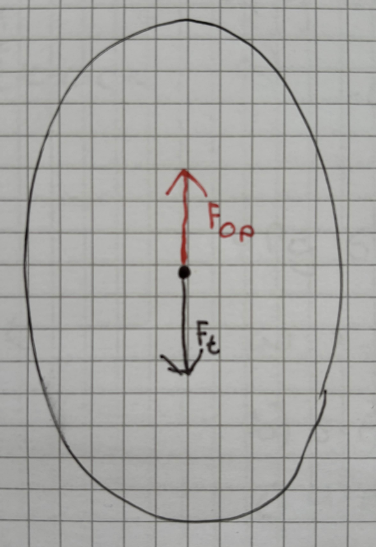
\includegraphics[width=0.3\textwidth]{figures/ballonskitse.png}
    \caption{Skitse af ballon med dens kræfter}
\end{figure}
Igen begynder vi med at skrive de brugbar værdier ned:
\\\\
Densiteten: \begin{math}1,20kg/m^3\end{math} \newline
Volume: \begin{math}3m^3\end{math} \newline
Ved brug af Archimedes' lov \begin{math}F_{op}=\rho\cdot V\cdot g\end{math}, kan man udregne opdriften der påvirker ballonen, tyngdeaccelerationen er stadig \begin{math}9,82 N/kg\end{math}
\begin{equation}
	F_{op}=1,20kg/m^3 \cdot 3m^3 \cdot 9,82N/kg=35,35N
\end{equation}

\subsection{Bestem temperaturen hvor ballonen letter når p = 1atm.}
For at ballonen skal kunne lette skal mængden af opdrift være større end hvad tyngdekraften skubbet ballonen ned.
\begin{equation*}
	F_{T_{Luft}} = F_{Op} - F_{T} = 35,35N - 1,08N = 34,27N
\end{equation*}

\begin{equation*}
	m_{luft} = \frac{F_{T_{Luft}}}{g} = \frac{34,27N}{9,82\frac{N}{kg}} = 3,49kg
\end{equation*}

\begin{equation*}
	\rho_{Luft} = \frac{m}{V} = \frac{3,49kg}{3m^{3}} = 1,16\frac{kg}{m^{3}}
\end{equation*}

\begin{equation*}
	T = \frac{M \cdot P}{R \cdot \rho} = \frac{0,029\frac{kg}{mol} \cdot 101,3kPa}{8,31\frac{Pa \cdot m^{3}}{mol \cdot K} \cdot 1,16 \frac{kg}{m^{3}}} = 303,96K
\end{equation*}